\documentclass[journal]{IEEEtran}

 
\usepackage{cite}

\usepackage{graphicx}
\usepackage{CJKutf8}

\ifCLASSINFOpdf  
\else
\fi






\hyphenation{op-tical net-works semi-conduc-tor}


\begin{document}

\begin{CJK*}{UTF8}{gbsn}


\title{基于领域驱动设计构建\\软件的学习}


%
%\author{ 作者: 朱信龙  \quad \quad  学号 :2017282110567 }
%

\markboth{ }
{Shell \MakeLowercase{\textit{et al.}}: Bare Demo of IEEEtran.cls for IEEE Journals}


\maketitle



\begin{abstract} 
  领域设计作为一种新的软件设计思想, 相对之前基于数据库驱动的
  开发方法,更强调了领域的概念,且架构清晰,对象职责分明, 可复用性好。 
  在系统开发的过程中,
  使用领域驱动的思想,可以大大提高开发效率,节约开发成本。
  可达到敏捷开发的目的。
  DDD其实是指一种分析方法,而不是(或者不主要是)设计方法。
  直白点说,就是设计项目之前要好好分析,而不是上来就做。
  DDD是分析的一套方法论。  
\end{abstract}


\begin{IEEEkeywords} 
  领域模型 ,领域驱动设计
\end{IEEEkeywords}



\IEEEpeerreviewmaketitle



\section{INTRODUCE}
 
在传统的系统开发中,软件开发人员与领域专家存在一
些隔阂,其根源就在于领域专家和软件开发人员使用两种截
然不同的语言。领域专家精通业务,喜欢使用自己的专业术
语,而软件开发人员则喜欢用面向对象的思维,习惯用代码
描述业务,从而造成了交流屏障,导致业务人员很难把需求。

传统的以数据库建模为核心的软件开发方法在基于 Web
多层架构的企业级应用系统开发中存在的诸多问题表现如
下:

\subsubsection {需求分析和设计不匹配}
分析阶段和设计阶段是断裂的(分析和设计人员通常是不同组别的两拨人)。
领域问题和技术问题的边界不清晰。
 
\subsubsection {围绕数据库的驱动设计}
开发人员一开始便根据需求建立数据库模型, 忽略面向对象的开发思想,业务逻辑设计混乱。
系统中的业务对象被机械化的数据库 CRUD 操作代替, 
代码的复用性和可维护性太差。大量写重复的代码。
所有操作的压力全部在数据库上,导致后期水平或者垂直扩展几乎要推到重来。
\\
\\ 针对以上的不足,将新阶段的领域驱动设计的开
发思想融入业务复杂的项目实践中,或许是一种不错的选择。




\subsection{Related work}
  领域驱动设计(Domain-Driven Design 简称 DDD)是一种
用来处理软件系统核心复杂性的方法。是以敏捷开发为手
段、以模型驱动设计为根基、以软件领域为着眼点的一种新
兴的软件开发方法,是一种新的面向对象的设计思想,也属
于模型驱动设计的一种。其核心部分是领域模型(Domain
model),是由一些定义的模型元素组成的,并使用分层架构
的方式来对业务逻辑进行隔离,领域问题内的所有业务逻辑
和规则都在这里反映出来,能对需求的变化做出快速的反
映。
\newline
\indent
  领域驱动设计抛弃了分裂分析模型与设计的做法,提出
要以通用语言作为开发中交流的统一语言,领域模型是通用
语言的基础,通用语言可以反映领域模型的本质,是开发人
员和领域专家之间有效沟通的工具。
\\

这里解释下一下通用语言和领域专家的意思,比如,不同部门的人对同一个概念有不同的角度。
通用语言的目的是让程序员和领域专家(领域专家就是天天用这个系统但是不是程序员的人,可以理解成甲方)之间对于项目中的概念(特别是名词和动词)达成一个一致的语言规范。

主要目的是消除歧义。例子:Cancel an order vs Delete a record。这两个对应的是同一个意思,只是领域专家和程序员用了不同的语言,所以通用语言的目的是让大家达成共识,以后交流的时候使用通用语言,譬如说只说*cancel an order**,也就是代码里面Order类下面只能由Cancel方法不能有Delete方法。

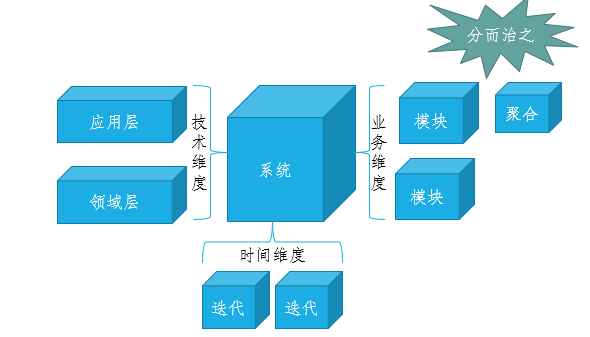
\includegraphics[scale=0.4]{2.png}
\subsubsection{为什么能应对复杂性}
采用DDD的设计思想,业务逻辑不再集中在几个大型的类上,而是由大量相对小的领域对象(类)组成,
这些类具备自己的状态和行为,每个类是相对完整的独立体,并与现实领域的业务对象映射。
领域模型就是由这样许多的细粒度的类组成。基于领域驱动的设计,
保证了系统的可维护性、扩展性和复用性,在处理复杂业务逻辑方面有着先天的优势。
\\
\subsubsection{为什么能应对快速变化}
一方面,项目中采用统一的语言进行交流,信息传达过程中,各方对问题的认识更容易保持一致;
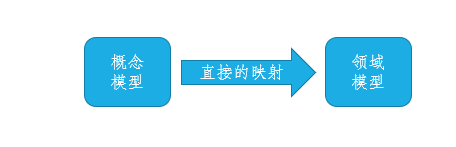
\includegraphics[scale=0.4]{1.png}

另一方面,业务模型直接映射领域模型,程序员看到领域模型代码,就看到业务需求。

\subsection{领域驱动设计的分层架构和构成要素}

下面我们简单介绍一下领域驱动设计的分层架构和构成要素,这部分内容在Eric Evans的书中有非常详尽的描述,想要详细了解的,最好去读原版书籍。

下面这张图是该书中著名的分层架构图,如下:

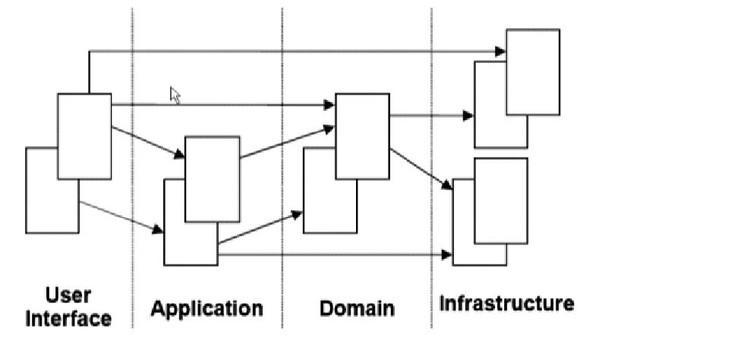
\includegraphics[scale=0.4]{3.jpeg}
\\

整个架构分为四层,其核心就是领域层(Domain),所有的业务逻辑应该在领域层实现,具体描述如下:
 
\subsubsection{用户界面层}
	负责向用户展现信息以及解释用户的输入。
\subsubsection{应用层}
  用来协调应用的活动。它不包含业务逻辑。它不保留业务对象的状态,但它保有应用任务的进度状态。
\subsubsection{领域层}
业务软件的核心所在。在这里保留业务对象的状态,对业务对象和它们状态的持久化被委托给了基础设施层。 


\subsubsection{基础设施层}
   为其他层的支撑库存在。它提供了层间的通信,实现对业务对象的持久化,包含对用户界面层的支撑库等作用。
   比如,各种中间件的使用。

\indent

下面详细介绍下领域模型的组成和设计规则:

\indent

一个领域模型有多个Aggregates组成。Aggregate划分了一堆class和其他class的一致性边界(Consistency Boundary)。

\indent

{\bfseries Aggregate}  之内强调一个事务一致性(transactional consistency),不同的Aggregates之间只要求最终一致(Eventual Consistency)。
  尽可能小的Aggregate。不需要一致性的东西尽量不要混进来。
  
\indent

{\bfseries Aggregate Root} 
是指在整个Bounded Context里面有全局Identity(就是唯一性标识)的类。
譬如说User, Company这种代表核心概念的类。
Aggregate Root本身也是一个Entity,不过是一个重要和特别的Entity。
Aggregate Root是操作整个Aggregate的入口。外界是通过Aggregate Root来操作这个Aggregate的。

\indent

{\bfseries   Entity }是指在一个Aggregate里面有唯一标识的类。
譬如说Address,一个User可以有好几个Address,这几个Address出了这个用户范围外后,就没有区分哪个是哪个的必要。
但是在这个用户之内,是要区分的,到底是家里的地址还是公司的地址。
判断两个Entities是否相等是看ID是否一样。
也就是Entity的属性一直处于可变的状态,但是还是一个Entity。
常见的例子就是Person,一个人的Age改变,Address改变,甚至Name改变,都是同一个人。
5岁的你和10岁的你是同一个人,只是你的状态一直在变。
哪怕两个人看起来一模一样,是双胞胎,他们还是不同的人,身份证的ID也不一样。这就是一个明显的Entity。
   
\indent 
{\bfseries Value Object} 
 
是指没有Identity的类,主要作为值来用。值是不变的,没有状态。譬如说Birthday,其实就是一个DateTime,没有什么Identity,大家在乎的就是里面的年月日是多少。
Value Object可以随意复制。
判断两个Value Objects是否相等是看所有的属性是否相等。

 




 \section{Conclusion}
对于领域驱动设计, 最核心的就是如何解决复杂
业务的设计问题,如何抓住业务逻辑的本质,并转换成
业务逻辑模型。领域驱动设计良好的支撑框架和富有
弹性的需求分析过程,已经得到业界的认可,  随着软件市场的
进一步成熟和客户需求的不断提高, 相信这是一个切
实可行且具有很好应用前景的开发方法。
\\
\indent
在项目实践应用领域驱动设计,一方面,切实感觉到了这种开发思想的自然,
更符合人的思考,不至于在业务复杂时写出一大堆不可复用的代码,自己给自己挖坑;
另一方面,还学习到了与之相关联的许多设计思想,感觉到了提升,让软件工程性的思想洗礼了一次,
以后应对复杂业务问题时,更能从容不迫。
{\bfseries  最后,由于是以前关于DDD的软件开发都为商用项目,不方便把项目中的一些东西写在报告里,
只能根据自己在做项目过程中,从书中和网络上学到的知识总结下来,望老师见谅。}


 
 


\section*{Acknowledgment}
感谢高级软件工程这门课,让我再次从工程的角度看待软件,对软件开发流程有了更清晰的认知;
对以前学习软件工程中的一些概念有了更深层的感悟,比如抽象,
组合,构造的思维,进行构件化,插件化开发。
要把高内聚,低耦合的思想融入到代码中,以便于重构和扩展。


\ifCLASSOPTIONcaptionsoff
  \newpage
\fi



\begin{thebibliography}{1}
 
 
\bibitem{IEEEhowto:kopka}
  《企业应用架构模式》,Martin Fowler著
\bibitem{IEEEhowto:kopka}
  《领域驱动设计—软件核心复杂性应对之道》,Eric Evans著 
\bibitem{IEEEhowto:kopka}
  《实现领域驱动设计》,Vaughn Vernon著
  
\end{thebibliography}

 
\clearpage
\end{CJK*}

\end{document}